% IEEE standard conference template; to be used with:
%   spconf.sty  - LaTeX style file, and
%   IEEEbib.bst - IEEE bibliography style file.
% --------------------------------------------------------------------------

\documentclass[letterpaper]{article}
\usepackage[T1]{fontenc}
\usepackage[utf8]{inputenc}
\usepackage{spconf,amsmath,amssymb,graphicx}
\usepackage[colorinlistoftodos]{todonotes}

\newcommand{\mytodo}[1]{\todo[inline]{#1}}
\newcommand{\dtodo}[1]{\todo[inline, color=cyan]{#1}}
\newcommand{\rtodo}[1]{\todo[inline, color=yellow]{#1}}
\newcommand{\ptodo}[1]{\todo[inline, nolist, color=green]{#1}}

% Example definitions.
% --------------------
% nice symbols for real and complex numbers
\newcommand{\R}[0]{\mathbb{R}}
\newcommand{\C}[0]{\mathbb{C}}

% bold paragraph titles
\newcommand{\mypar}[1]{{\bf #1.}}

% Title.
% ------
\title{Optimizing Simplex Implementation For Standard Form Problems}
%
% Single address.
% ---------------
\name{Donjan Rodic, Rico Häuselmann} 
\address{Department of Mathematics\\ ETH Zürich\\Zürich, Switzerland}

% For example:
% ------------
%\address{School\\
%		 Department\\
%		 Address}
%
% Two addresses (uncomment and modify for two-address case).
% ----------------------------------------------------------
%\twoauthors
%  {A. Author-one, B. Author-two\sthanks{Thanks to XYZ agency for funding.}}
%		 {School A-B\\
%		 Department A-B\\
%		 Address A-B}
%  {C. Author-three, D. Author-four\sthanks{The fourth author performed the work
%		 while at ...}}
%		 {School C-D\\
%		 Department C-D\\
%		 Address C-D}
%

\begin{document}
%\ninept
%
\maketitle
%

\begin{abstract}
We implement Dantzigs Simplex Algorithm for Linear Programming, a widespread and established linear optimization method.
Various computational optimization techniques are used to improve the efficiency of the algorithm and explore the options of improving upon this highly memory-bound problem;
and to compare it to well-known industry tools.
Our specific focus on the sub-class of feasible standard maximization problems allows us to achieve performance close to the hardware maximum.
\end{abstract}

%%%%%%%%%%%%%%%%%%%%%%%%%%%%%%%%%%%%%%%%%%%%%%%%%%%%%%%%%%%%%%%%%%%%%%%%%%%%%%%%
%%%%%%%%%%%%%%%%%%%%%%%%%%%%%%%%%%%%%%%%%%%%%%%%%%%%%%%%%%%%%%%%%%%%%%%%%%%%%%%%

\section{Introduction}\label{sec:intro}

In this section we will motivate our choice of algorithm to optimize and give
a brief overview of related work.

\mypar{Motivation} The Simplex algorithm for linear optimization is widely
used in logistics, optimization of business performance and many other fields.

The simplex solution to linear problems (LPs) may be used as a crucial part in
basic decision making wherever management requirements for interdependent resources produce linear constraints.
In production environments performance is often crucial, therefore it is interesting to see how far
a solver for a specific class of linear problems can be optimized.

\mypar{Implementation} We present an implementation which is geared towards 
a limited class of linear optimization problems and solves this kind of problem
faster than any commercially available general purpose solver.

\mypar{Related work} Many production grade linear optimization packages exist.
We used a number of them to compare the performance of our implementation to what is being
used in big business.
\begin{itemize}
    \item{GLPK \cite{glpk}, a free open source linear programming package.}
    \item{Gurobi \cite{gurobi}, a commercial grade package which claims to be the fastest available solution when taking into account multi-threading. Gurobi is free for educational use.}
    \item{SoPlex \cite{soplex}, free for educational use, developed at Zuse Institute Berlin (ZIB).}
    \item{CPPLEX \cite{cpplex}, a free open source mathematical implementation emphasizing clean object oriented code style.}
\end{itemize}

%%%%%%%%%%%%%%%%%%%%%%%%%%%%%%%%%%%%%%%%%%%%%%%%%%%%%%%%%%%%%%%%%%%%%%%%%%%%%%%%
%%%%%%%%%%%%%%%%%%%%%%%%%%%%%%%%%%%%%%%%%%%%%%%%%%%%%%%%%%%%%%%%%%%%%%%%%%%%%%%%

\section{Background: The Simplex Algorithm}\label{sec:background}
It follows a brief introduction to the class of problem in consideration
and the algorithm used as well as a cost analysis of the algorithm.

\mypar{Linear Optimization Problems \cite{dantzig}}
The general formulation of a linear problem is
\begin{eqnarray*}
    \max c^T x, & \text{Subject To}\\
    b_l \leq A x \leq b_u,
\end{eqnarray*}
Where $c \in \mathbb{Q}^n$, $x \in \mathbb{R}^n$, $A \in \mathbb{Q}^{m \times n}$ and $b \in \mathbb{R}^m$.

\mypar{Standard form Linear Problems}
A linear problem is considered to be in standard form when it is formulated as
\begin{eqnarray*}
    \max c^T x, & \text{Subject To}\\
    A x \leq b \\
    x \geq 0.
\end{eqnarray*}
Any linear problem can be transformed into standard form \cite{groetschel}. 
Considering this we chose to restrict our solver to standard form problems, since supporting other formulations would have lead to more effort being put into transforming the problem into standard form (effectively implementing a domain specific language).

\mypar{The Simplex Method}
The tableau form of the simplex method for standard form problems works as follows:
Let $m$ be the number of constraints and $n$ the number of variables.
\begin{enumerate}
    \item initialize the tableau $T \in \mathbb{R}^{(m+1) \times (n+m+1)}$
        \[ T = 
            \left[
            \begin{matrix}
                A & I_m & b \\
                c & 0 & 0
            \end{matrix}
            \right]
        \]
        And create a set of column indices to keep track of the currently ``active'' columns (also called the basis). 
        Initialize the basis with the indices 
        \[ B = \{ m, \dots, n+m-1 \} \]
    \item iterate:
        \begin{enumerate}
            \item (Pivoting) If $\nexists\, i\, |\, T_{m,i} < 0$ problem is solved. Else:
                \[\text{pcol} := \text{argmin}\left(T_{m,i}\right)\]
            \item (Pivoting) If $\nexists\, i\, |\, T_{i, \text{pcol}} > 0$ problem is infeasible. Else:
                (Basis Exchange)\[\text{prow} := \text{argmin}\left(\frac{T_{i, 2m}}{T_{i,\text{pcol}}} \right)\]
            \item perform Gaussian elimination:
                \[p :=  T_{\text{prow}, \text{pcol}}\]
                for $i \in \{0, \dots, m-1\}$:
                \[ T_{i,:} := T_{i,:} - T_{\text{prow},:} \frac{T_{i,\text{pcol}}}{p},\, if\, i \neq \text{prow}, \]
                and update the basis
                \[ B := B \setminus \{\text{prow}\} \cup \{\text{pcol}\}. \]
        \end{enumerate}
\end{enumerate}

\mypar{Cost Analysis}
The cost of the overall algorithm depends highly on the coefficients of the problem,
since the coefficients determine the number of iterations necessary. 
A small problem may very well take more iterations to solve than a huge one.

However, the number of operations contained in one iteration only depends on the problem size.
Let the number of iterations be $N$, then
\[ \text{\#flops} = N \times 2 m \times (m + n + 1) \]
As well as the number of doubles read from memory, which bounded from below by
\[ \frac{(m + 1) \times (m + n + 1)}{B} \leq \text{\#loads}, \]
Where $B$ is the block size of the L1 cache for very small problems where the entire
tableau fits into cache, and bounded from above by
\[ \text{\#loads} \leq N \times (3m + n) + (m + 1) \times (m + n + 1), \]
Assuming every load is a miss.

For the operational intensity this means:
\[ \frac{1}{4} \leq I \leq \frac{B\times N}{4} \]

%%%%%%%%%%%%%%%%%%%%%%%%%%%%%%%%%%%%%%%%%%%%%%%%%%%%%%%%%%%%%%%%%%%%%%%%%%%%%%%%
%%%%%%%%%%%%%%%%%%%%%%%%%%%%%%%%%%%%%%%%%%%%%%%%%%%%%%%%%%%%%%%%%%%%%%%%%%%%%%%%

\section{Our Implementation}\label{sec:yourmethod}

In this section we explain the our baseline implementation as well as all optimizations we made.

\mypar{Baseline Implementation}
Our baseline implementation parses an input file containing the coefficients for the objective function and the constraints.
It assumes the problem is in standard form and that the number of constraints is even.
The coefficients are stored in a two dimensional STL vector of vector representation of the simplex tableau.

The steps performed in each iteration are separated into three functions: 
\begin{itemize}
    \item{\tt pivot\_col}
    \item{\tt pivot\_row}
    \item{\tt base\_exchange}
\end{itemize}
The first two contain the code for finding the pivot element to use in the iteration whereas
the third facilitates the Gaussian elimination step.

\mypar{Profiling}
Profiling was done with {\tt gprof}, {\tt perf} and {\tt valgrind}. All tools consistently showed that the vast majority of the
runtime is spent in the {\tt base\_exchange} function, where we focused all subsequent optimization.
Further annotated analysis revealed stalls at the memory access functions, which can be alleviated by exploiting instruction level parallelism (ILP) via static scalar assignment
where unit stride access was applicable.


\mypar{Array}
The Array optimization replaces the vector of vectors implementation of the tableau by
a C99 one dimensional contiguous array allocated and aligned using {\tt \_mm\_malloc} from
the Intel intrinsics headers.

All subsequent optimizations were based on this implementation.

\mypar{SSA}
The first optimization consisted of unrolling the tightest loop and applying static assignment in order to increase ILP.

\mypar{Blocking}
As a next step we added blocking in the loop that runs over the whole tableau 
inside the basis exchange. Block sizes from $1 \times 1$ to $16 \times 16$ were tried.

The code for different block sizes was generated using 
{\tt cheetah} \cite{cheetah}, a templating engine for python. The following optimizations were introduced
by changing the code templates to be able to make use of the best block size.

\mypar{Cache control}
Improvement of cache access attempted through intrinsics for non temporal assignment, in order to avoid polluting the cache with updates on the active basis elements and
effective cost calculations. We further added prefetching in order to load soon-to-be-used blocks into the L2 cache, as well as prefetching parts of the current block into L1.

\mypar{Swapping}
In order to allow the compiler to perform optimization much better, the pivot and the last row
of the tableau were swapped before and after entering the main loop of the base exchange step,
allowing to get rid of the if statements used to test for the pivot row in the main loop.

This optimization does not change the number of floating point operations performed, however it affects the number of bytes loaded per iteration slightly.

\mypar{Vectorization}
In the last phase, manual vectorization using advanced vector extensions (AVX) instructions was performed.

%%%%%%%%%%%%%%%%%%%%%%%%%%%%%%%%%%%%%%%%%%%%%%%%%%%%%%%%%%%%%%%%%%%%%%%%%%%%%%%%
%%%%%%%%%%%%%%%%%%%%%%%%%%%%%%%%%%%%%%%%%%%%%%%%%%%%%%%%%%%%%%%%%%%%%%%%%%%%%%%%

\section{Experimental Results}\label{sec:exp}

We give a short overview of our hardware and software framework, followed by measurements and visualization of the code performance.

\mypar{Experimental setup}
All experiments were conducted on a Core i5-3360M (Ivy Bridge) running GNU/Linux and 32 kB L1 cache, 256 kB L2 cache and 3 MB L3 cache, all at 64 bytes line size.

GCC 4.7.3 was used for compilation. The following flags were used:
{\tt -O3 -march\--native  } for automatic vectorization with {\tt -fno\--tree\--vectorize \\ -fno\--tree\--slp\--vectorize -mno\--abm } additionally for non vectorized code.
For profiling {\tt -g3 -ggdb -pg } was added. Turboboost has been taken care of.

A random linear problem generator was written to test the implementations. 
The problem generator is restricted for simplicity's sake to generate problems with guaranteed feasibility by allowing only positive coefficients. 
The same parameter was used for the number of Variables as well as the number of constraints.

The problem size was varied from 10 to 1000, or up to 4000 where relevant for out-of-cache comparison.
Due to the unpredictable count of steps the Simplex algorithm needs to reach a solution, each problem size was averaged over up to 100 samples.
Additionally, in order to achieve a defined minimum of RDTSC cycles, small problems were repeatedly calculated as shown in the exercise framework.

The code was instrumentalized to count floating point and memory operations. The measured numbers for both were compared to manually computed values and found to agree.

In order to compare to third party packages, their respective application programming interface (API) was used according to the available documentation. 
The same technique was used to measure runtime, however instrumentalization was not used.
We used Gurobi \cite{gurobi}, SoPlex \cite{soplex}, GLPK \cite{glpk} and CPPLEX \cite{cpplex}, with the last one being dropped from testing because of numerical instability for large problems.

%%%%%%%%%%%%%%%%%%%%%%%%%%%%%%%%%%%%%%%%%%%%%%%%%%%%%%%%%%%%%%%%%%%%%%%%%%%%%%%%

\mypar{Results}

Direct comparison with alternative Simplex solvers (see Fig.~\ref{res_external}) shows that even our baseline implementation performs significantly faster than any of the alternatives.
This results from the simplicity assumptions we have made (regularity, conformity, definiteness) under which a lot of tedious checks can be eliminated.
Unfortunately none of the APIs offered to impart this information to the respective solver.
We plot the elapsed RDTSC cycles instead of per cycle performance so as not to guess the operation count of each solver.

\begin{figure}\centering
  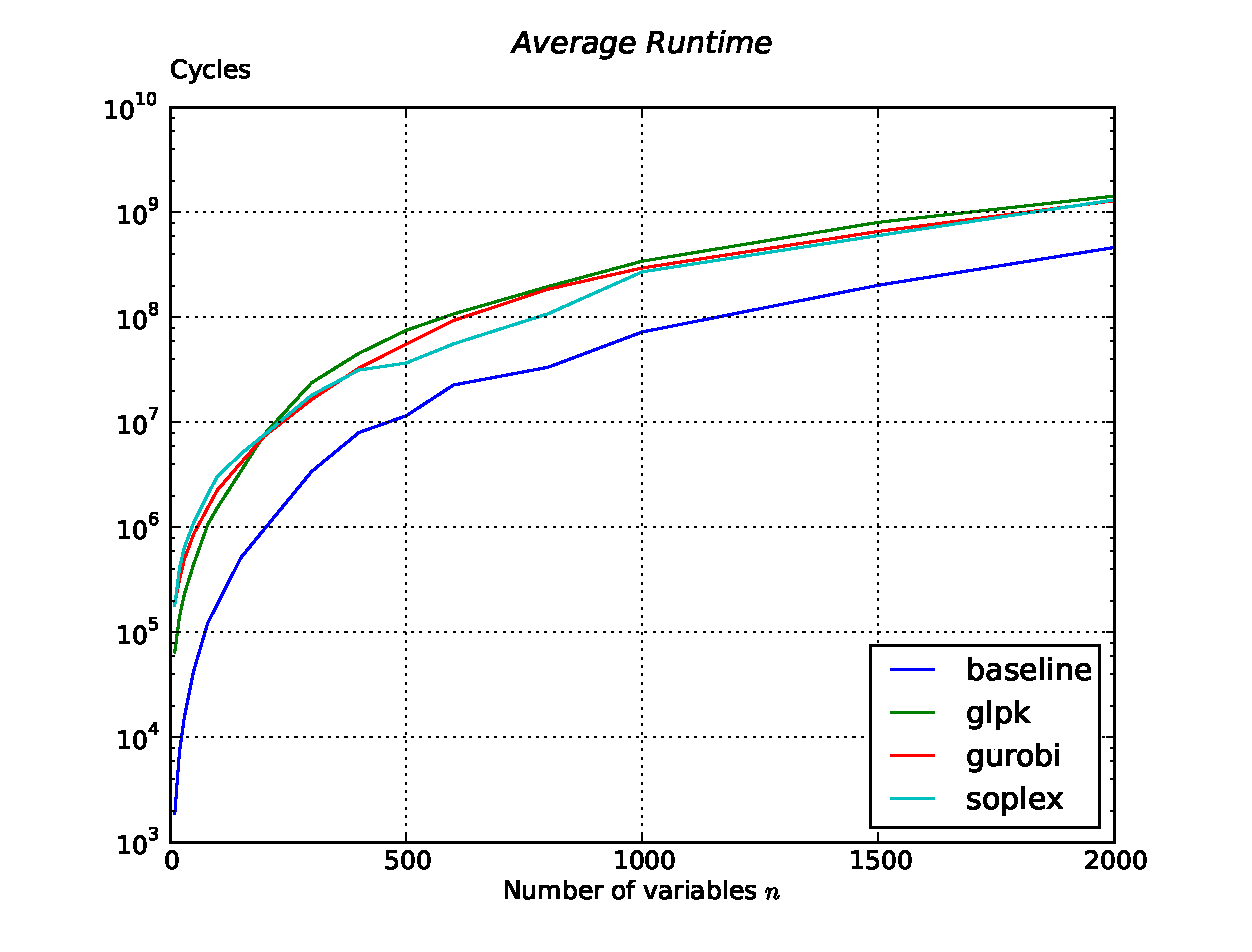
\includegraphics[scale=0.4]{img/results_compare_external.eps}
  \caption{Comparison with Gurobi, SoPlex and GLPK.\label{res_external}}
\end{figure}


Of our own optimization techniques, blocking with an additional copy (swap) step showed to be the most efficient for large sizes,
both non-auto-vectorized (Fig.~\ref{res_basic_novec}) and auto-vectorized (Fig.~\ref{res_basic_autovec}).
Note that while in theory an AVX enabled program could reach 8 flop/cycle for compute-bound problems on our testing machine, the plots have been capped at 2 flop/cycle for better readability.
All further plots contain programs with approximately the same operation count.

\begin{figure}\centering
  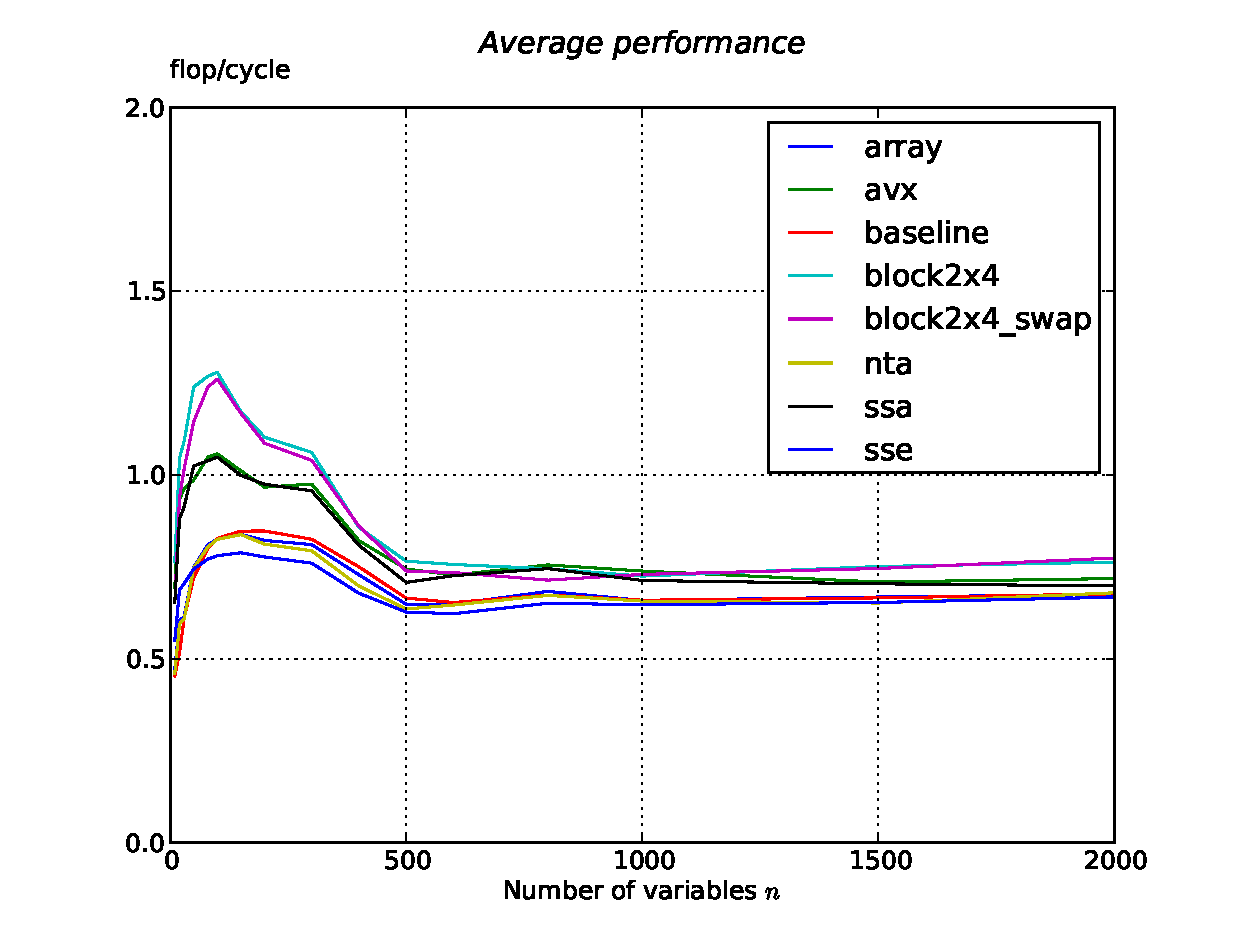
\includegraphics[scale=0.4]{img/results_basic_novec.eps}
  \caption{Non-auto-vectorized basic implementations.\label{res_basic_novec}}
\end{figure}

\begin{figure}\centering
  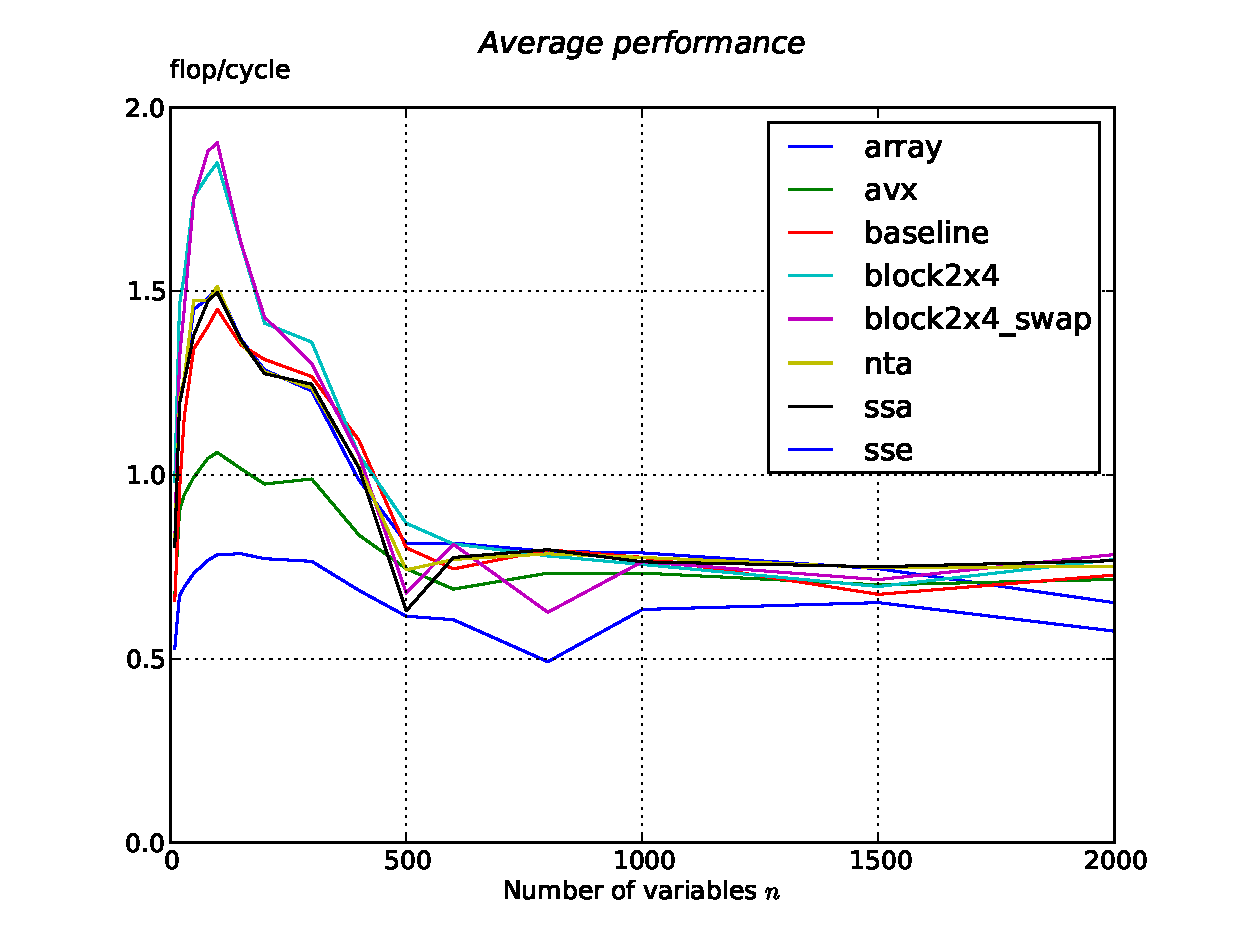
\includegraphics[scale=0.4]{img/results_basic_autovec.eps}
  \caption{Auto-vectorized basic implementations.\label{res_basic_autovec}}
\end{figure}


Our further goal was to find the optimal block sizes by varying unrolling width and concurrent line elimination count.
The search space consisted of the dyadic product of these two parameters for the dyadic product of AVX and scalar code
as well as blocking and non-blocking versions and incidentally turned out to favor our originally picked sizes.

\begin{figure}\centering
  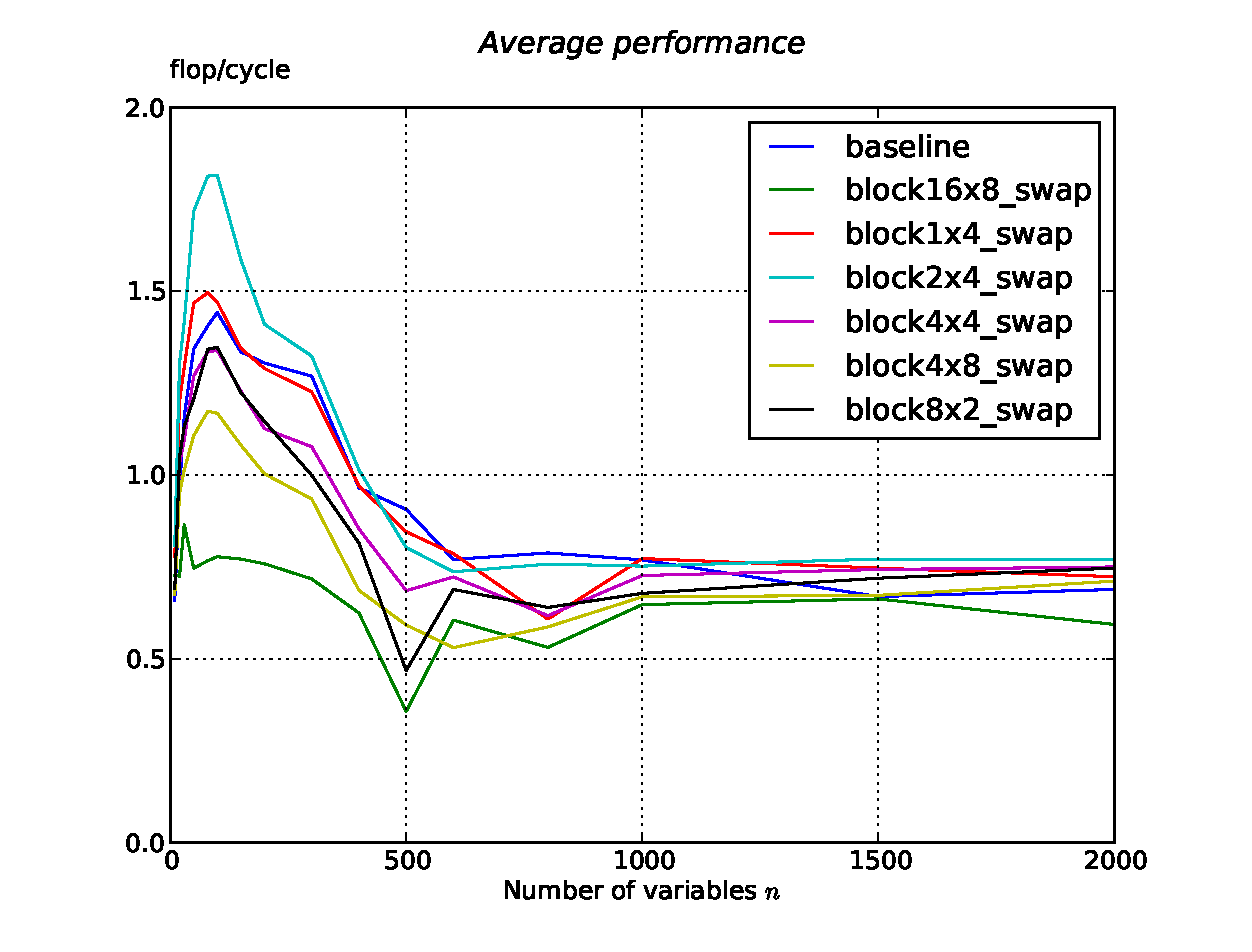
\includegraphics[scale=0.4]{img/results_find_blocks.eps}
  \caption{A small selection of the parametrized blocking implementations. Note the kink around $n=500$, which may indicate a numerically particularly challenging problem.\label{res_findblock}}
\end{figure}

For large problems, our most efficient blocking algorithm achieves 0.75 flop/cycle, compared to the baseline 0.68 flop/cycle.
Small problems that fit in cache are at the show the greatest difference around $n=100$ with 1.83 flop/cycle for the blocking algorithm and 1.46 flop/cycle for the baseline.
These correspond to speedups of 25\% respectively 10\%, although we drop to hardly any speedup at the cache boundaries.

Could we improve on this further?
As shown in Fig.~\ref{fig:res_cachecontrol}, combining our previous favorite with non temporal assignment resulted in a mostly positive but small effect on the swapping implementations.
Any kind of manual prefetching as described in section 3, or partial implementations thereof, lead to a considerable slowdown.

\begin{figure}\centering
  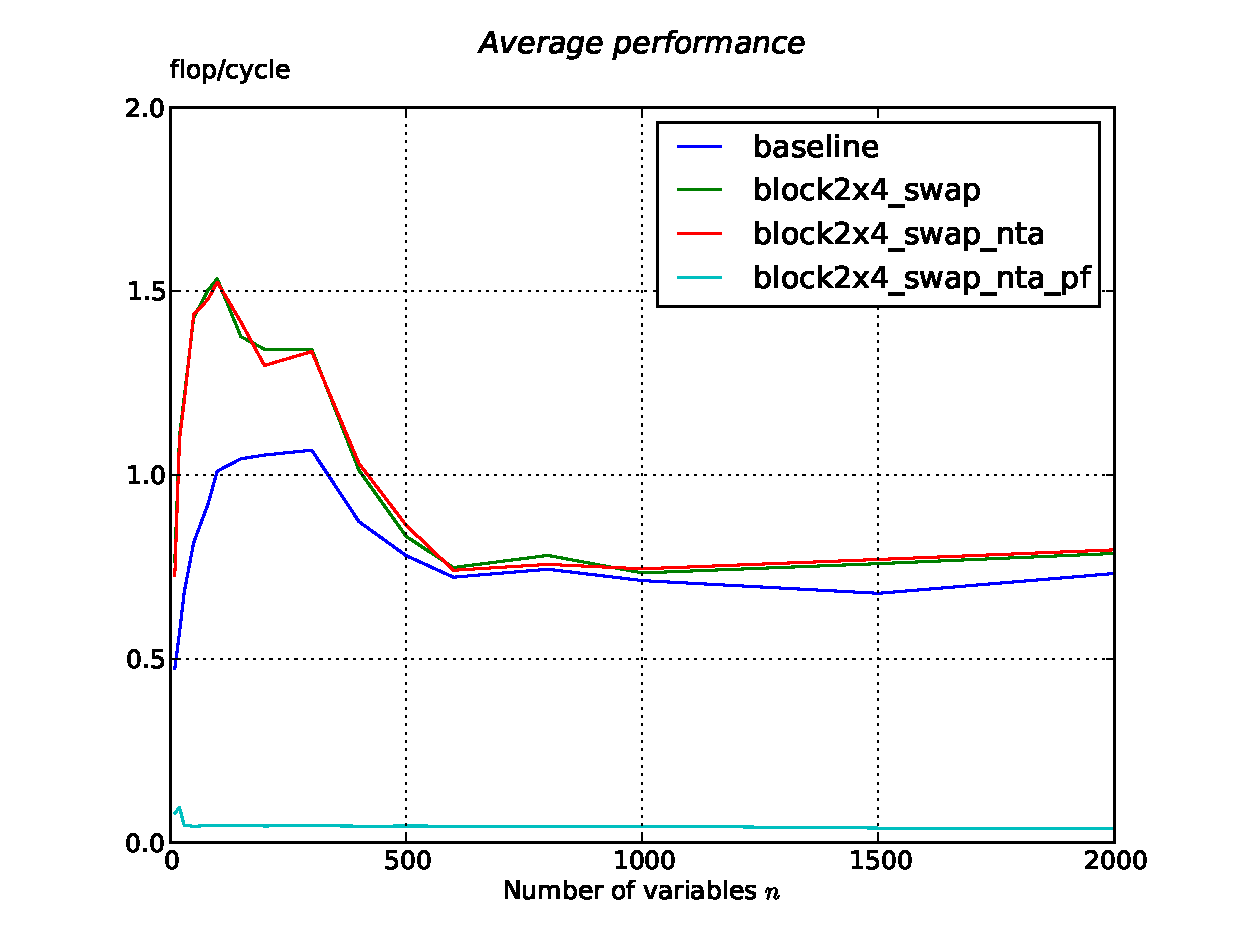
\includegraphics[scale=0.4]{img/results_cachecontrol_novec.eps}
  \caption{Performance of non temporal assignment ({\tt \_nta}) and prefetching ({\tt \_nta\_pf}) implementations of {\tt block2x4\_swap} and the baseline.\label{fig:res_cachecontrol}}
\end{figure}

One particularly interesting result is that the effect of AVX intrinsics on performance is not easy to predict if we turn on auto-vectorization,
yet they do not match the fastest auto-vectorized version (Fig.~\ref{fig:res_avx}).

\begin{figure}\centering
  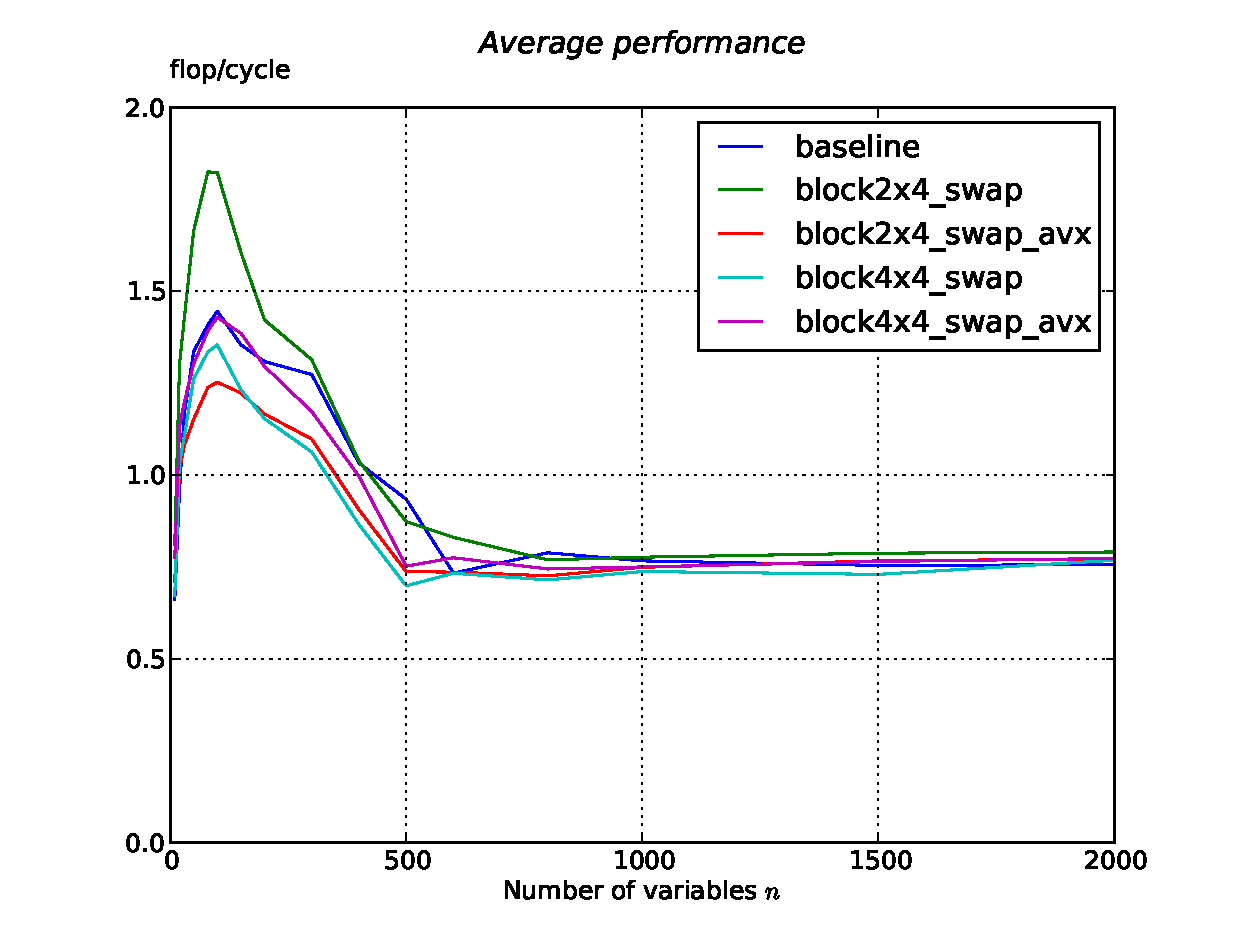
\includegraphics[scale=0.4]{img/results_avx.eps}
  \caption{Example comparison of auto-vectorized code and its AVX counterpart.\label{fig:res_avx}}
\end{figure}

Profiling of the {\tt swapNxM\_block\_avx } implementations showed that between 70\% and 90\% of the time is spent on {\tt \_mm256\_load\_pd } calls,
which once more underlines the memory tightness of the problem.

From the roofline plot shown in Fig.~\ref{fig:res_roof_high} we learn that our best-performing implementation is very close to the theoretical memory limit.
The corresponding test set starts with problems of size 500 in order to measure only RAM to CPU traffic.

\begin{figure}\centering
  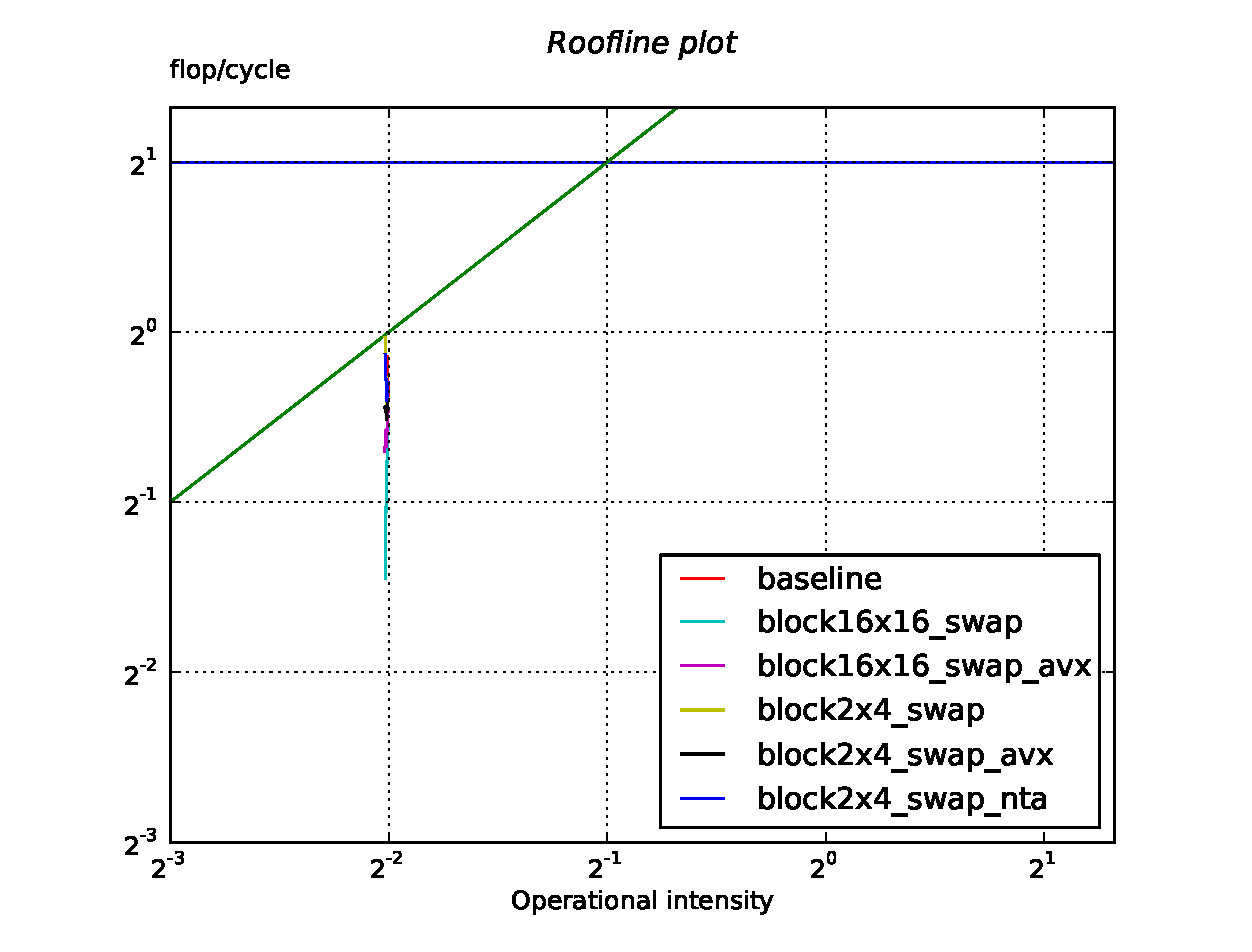
\includegraphics[scale=0.4]{img/roof_high_autovec.eps}
  \caption{Roofline plot, the 8 flop/cycle performance line is cropped away for better readability.\label{fig:res_roof_high}}
\end{figure}


%%%%%%%%%%%%%%%%%%%%%%%%%%%%%%%%%%%%%%%%%%%%%%%%%%%%%%%%%%%%%%%%%%%%%%%%%%%%%%%%
%%%%%%%%%%%%%%%%%%%%%%%%%%%%%%%%%%%%%%%%%%%%%%%%%%%%%%%%%%%%%%%%%%%%%%%%%%%%%%%%

\section{Conclusions}

Our measurement results and profiling indicate that the problem is highly memory bound and at the same time keeps
a very simple structure, which does not lend itself to optimization easily.
We were able to realize a speedup of up to 25\% for small problems and up to 10\% for large ones.

Finally, we can conclude that in cases where many linear problems of only one certain 
class has to be solved and performance matters it might pay to invest into a specifically
tailored solution. Depending on the restrictions of the problem class loss of generality
may be rewarded with great speed gains.

%%%%%%%%%%%%%%%%%%%%%%%%%%%%%%%%%%%%%%%%%%%%%%%%%%%%%%%%%%%%%%%%%%%%%%%%%%%%%%%%
%%%%%%%%%%%%%%%%%%%%%%%%%%%%%%%%%%%%%%%%%%%%%%%%%%%%%%%%%%%%%%%%%%%%%%%%%%%%%%%%



% References should be produced using the bibtex program from suitable
% BiBTeX files (here: bibl_conf). The IEEEbib.bst bibliography
% style file from IEEE produces unsorted bibliography list.
% -------------------------------------------------------------------------
\bibliographystyle{IEEEbib}
\bibliography{bibl_conf}

\end{document}

